% CVPR 2027 submission (review version); built on the official cvpr-org author kit.
% Build: latexmk -pdf -interaction=nonstopmode -halt-on-error main.tex   (or ./build.sh)

\documentclass[10pt,twocolumn,letterpaper]{article}

%%%%%%%%% PAPER TYPE
% \usepackage{cvpr}              % To produce the CAMERA-READY version
\usepackage[review]{cvpr}      % To produce the REVIEW version
% \usepackage[pagenumbers]{cvpr} % To force page numbers, e.g. for an arXiv version

% Import additional packages in the preamble file, before hyperref
%% Preamble shared by main.tex and supp.tex.
%% Kit tweaks (cvpr-org author kit, CVPR 2027) followed by project packages and macros.

%%
%% Inline annotations; for predefined colors, refer to "dvipsnames" in the xcolor package
%%
\newcommand{\red}[1]{{\color{red}#1}}
\newcommand{\todo}[1]{{\color{red}#1}}
\newcommand{\TODO}[1]{\textbf{\color{red}[TODO: #1]}}
%%
%% disable for camera ready / submission by uncommenting these lines
%% (do this only after every \TODO has been resolved in the text itself)
%%
% \renewcommand{\TODO}[1]{}
% \renewcommand{\todo}[1]{#1}

%%
%% Commonly used math definitions
%%
\DeclareMathOperator*{\argmin}{arg\,min}
\DeclareMathOperator*{\argmax}{arg\,max}
\DeclareMathOperator{\softmax}{softmax}
\DeclareMathOperator{\sg}{sg}

%%
%% Project packages (cvpr.sty already loads xcolor, graphicx, amsmath, amssymb, booktabs)
%%
\usepackage{booktabs}
\usepackage{multirow}
\usepackage{xcolor}
\usepackage{graphicx}
\usepackage{amsmath}
\usepackage{amssymb}
\usepackage{makecell}

%%
%% Results. NO NUMBER FOR A NEW EXPERIMENT IS TYPED BY HAND.
%% Every new measurement enters through \res{key}; the keys are written to
%% generated/results.tex by scripts/analyze_results_c11.py
%% (python scripts/run_c11_matrix.py --matrix ... analyze). A missing key prints a red TBD.
%%   \res{<variant>@<split>@<metric>}          mean over seeds
%%   \res{<variant>@<split>@<metric>@pm}       mean {\scriptsize +- std}
%%   \res{<variant>@<split>@<metric>@std}
%%   \res{<variant>@<split>@nseeds}
%%   \res{cmp@<variant>@<control>@<split>@<metric>@diff|ci|wins|p}
%% split  in {validation, test}
%% metric in {mpjpe (H36M joint-0 root), mpjpehip (J14 hip-midpoint root), pampjpe,
%%            pve (historical, unaligned), pvepelvis (minus H36M joint 0),
%%            pvehip (minus J14 hip midpoint), accel (mm/frame^2), accelms (m/s^2, 30 fps)}
%% Reference checkpoints use seed 0: P-parent, R-c10-archived, R-c00-archived.
%%
\newcommand{\res}[1]{\ifcsname res@#1\endcsname\csname res@#1\endcsname\else\textcolor{red}{\textbf{TBD}}\fi}
\robustify{\res}
\InputIfFileExists{generated/results.tex}{}{}

%% Shorthands for paired comparisons: {variant}{control}{split}{metric}
\newcommand{\cmpdiff}[4]{\res{cmp@#1@#2@#3@#4@diff}}
\newcommand{\cmpci}[4]{\res{cmp@#1@#2@#3@#4@ci}}
\newcommand{\cmpwins}[4]{\res{cmp@#1@#2@#3@#4@wins}}
\newcommand{\cmpp}[4]{\res{cmp@#1@#2@#3@#4@p}}
%% Table cell: difference with its 95% CI underneath-size
\newcommand{\dci}[4]{\cmpdiff{#1}{#2}{#3}{#4}\,{\scriptsize\cmpci{#1}{#2}{#3}{#4}}}
%% Running-text form: "Delta = d mm (95% CI [lo, hi]; w sequences)"
\newcommand{\dtext}[4]{\mbox{$\Delta{=}$\cmpdiff{#1}{#2}{#3}{#4}\,mm} (95\% CI \mbox{\cmpci{#1}{#2}{#3}{#4}}; lower on \cmpwins{#1}{#2}{#3}{#4} sequences)}

%% Variant names used in the text and tables
\newcommand{\vA}[1]{\textsf{A#1}}
\newcommand{\vB}[1]{\textsf{B#1}}
\newcommand{\vC}[1]{\textsf{C#1}}
\newcommand{\method}{STaR-Body\xspace}

%% Data figures produced after the experiments (scripts/make_c11_figures.py).
%% \genfig{basename}{width}{fallback height}
\newcommand{\genfig}[3]{%
  \IfFileExists{figures/generated/#1.pdf}%
    {\includegraphics[width=#2]{figures/generated/#1.pdf}}%
    {\fbox{\parbox[c][#3][c]{\dimexpr#2-2\fboxsep-2\fboxrule\relax}{\centering\footnotesize\color{red}%
      \textbf{figures/generated/#1.pdf}\\figure generated by\\\texttt{scripts/make\_c11\_figures.py}\\after experiments}}}}

%%
%% Fine-tune spacing (kit options)
%%
\setlength{\abovecaptionskip}{.4em}


\definecolor{cvprblue}{rgb}{0.21,0.49,0.74}
\usepackage[pagebackref,breaklinks,colorlinks,allcolors=cvprblue]{hyperref}

\def\confName{CVPR}
\def\confYear{2027}

%%%%%%%%% TITLE
\title{STaR-Body: Identity-Preserving Evidence Routing\\for Spatiotemporal Human Mesh Refinement}

%%%%%%%%% AUTHORS (anonymous for review)
\author{Anonymous CVPR submission}

\begin{document}
\maketitle
\begin{abstract}
Video human mesh refiners routinely condition on 2D keypoints, yet the interface through which this evidence reaches the body is rarely isolated: keypoints are pooled or concatenated into one vector that is broadcast to every joint.
We ask whether preserving the identity of each landmark and routing it to the joints it constrains matters once the evidence is real.
An audit of our own joint-indexed feedback motivates the question: its landmark observations came from a head that never received gradient, so it routed drift from a frozen reference model rather than image evidence.
\method therefore turns external detector keypoints into identity-bearing tokens that carry the residual to the current body projection, the projection itself and the detector confidence.
Twenty-four SMPL joint queries read these tokens through attention with a kinematic-tree distance bias; the feedback is recomputed at every refinement iteration, enters before part pooling and masked temporal exchange, and starts from a zero-initialised output that preserves the inherited prediction.
On 3DPW, all variants start from one parent, share a 1,000-step budget and three seeds, and are tested once through validation locks; we compare routing with no feedback, capacity-matched pooling, ordered-vector conditioning, identity-free sets, unbiased and wrongly biased routing, and a weaker detector, using paired intervals that combine seed and test-sequence variance.
\TODO{One sentence with the main test result, \eg ``Routing lowers test MPJPE by \cmpdiff{B4-ext-joint}{B7-ext-concat}{test}{mpjpe}\,mm relative to ordered-vector conditioning (95\% CI \cmpci{B4-ext-joint}{B7-ext-concat}{test}{mpjpe})''; if the CIs include zero, state that identity-preserving routing performs on par with global conditioning and summarise what does matter.}
\end{abstract}

\section{Introduction}
\label{sec:intro}

Monocular human mesh recovery estimates an articulated SMPL body~\cite{loper2015smpl} from images.
Single-image regressors~\cite{kanazawa2018hmr,kolotouros2019spin,goel2023hmr2} now provide strong initial estimates, and video methods refine them with temporal context~\cite{kocabas2020vibe,choi2021tcmr,shen2023glot} and with detected 2D keypoints~\cite{shin2024wham,shen2024gvhmr}.
Keypoints are an attractive refinement signal: they are cheap to obtain from mature detectors~\cite{cao2021openpose,xu2022vitpose}, they are expressed in the same image plane as the body projection, and each of them constrains a specific part of the kinematic tree.
How this evidence should \emph{enter} a refiner, however, is rarely studied in isolation.
Common interfaces pool landmark residuals into a single vector or concatenate the keypoints into an ordered per-frame vector; either way, a single per-frame feature computed by a global network conditions every joint.
Pooling discards which landmark produced a residual, and concatenation keeps identity only by position, leaving a global network to discover which joint each coordinate should move.

This paper asks a narrow question: \emph{does preserving landmark identity, and routing each landmark anatomically to the joints it constrains, matter once the evidence is real?}
We were led to it by an audit of our own earlier refiner.
An earlier variant of our refiner routed 17 landmark tokens to 24 joint queries and reported small single-seed validation gains over a mean-feedback control (PVE 72.82 \vs 73.05\,mm).
Its landmark observations, however, came from an observation head whose 2D losses were zero in every training stage; the head never left its initialisation and its output equals the projection of the frozen reference model (\cref{sec:audit}; \TODO{confirm}).
That refiner therefore routed the drift of the current body from a frozen reference, not image evidence, and its mean control had 206 times fewer parameters.
The earlier comparison cannot answer the question above.

We therefore rebuild the feedback interface around external detector keypoints and design a study that changes one factor at a time.
\method encodes each ViTPose~\cite{xu2022vitpose,xu2024vitposepp} landmark as a token that carries its residual to the current body projection, the projection itself, its detector confidence and a learned identity embedding.
Twenty-four SMPL joint queries read these tokens through multi-head attention with a soft kinematic-tree distance bias.
The routed feedback is recomputed at every refinement iteration as the body moves, enters each joint before anatomical part pooling and masked temporal exchange, and is zero at initialisation, so every variant starts from exactly the inherited prediction (\cref{fig:overview}).
Around this router we place controls that isolate the evidence source (none, self-referential, external), the interface (capacity-matched pooling, ordered concatenation, identity-free set attention, routing), the anatomical prior (none, correct, deranged) and the evidence quality (ViTPose \vs the OpenPose~\cite{cao2021openpose} detections shipped with 3DPW~\cite{vonmarcard2018pw3d}).
All variants start from one parent checkpoint, share a 1,000-step budget and a pre-registered evaluation step, are trained with three seeds, and are evaluated on the 3DPW test split exactly once through immutable validation locks.

Our contributions are
(i)~a diagnostic showing that joint-indexed feedback built on an untrained observation head routes reference drift, which explains why an apparent interface effect can arise without image evidence;
(ii)~an identity-preserving evidence router that turns external keypoints into anatomically routed, per-iteration joint feedback inside a spatiotemporal refiner, with bounded rotation updates and a start that reproduces the inherited prediction exactly;
and (iii)~a controlled, multi-seed study with paired sequence-clustered statistics that separates evidence, identity, routing, anatomical prior and evidence quality.
\TODO{Close the paragraph with the answer once test numbers exist, \eg ``Routing real evidence improves over ordered-vector conditioning and pooling on the 3DPW test split, whereas routing self-referential evidence does not''; if routing is not distinguishable from global conditioning, say so and state the finding that does hold (\eg evidence source matters more than interface).}

\section{Related Work}
\label{sec:related}

\paragraph{Regression and geometric feedback.}
HMR~\cite{kanazawa2018hmr}, SPIN~\cite{kolotouros2019spin} and HMR\,2.0~\cite{goel2023hmr2} established direct SMPL regression; CLIFF~\cite{li2022cliff} and CameraHMR~\cite{patel2025camerahmr} add full-frame and perspective cues, while BEDLAM~\cite{black2023bedlam} shows the value of synthetic training data.
PARE~\cite{kocabas2021pare} attends to body parts, and PyMAF~\cite{zhang2021pymaf}, PyMAF-X~\cite{zhang2023pymafx} and ReFit~\cite{wang2023refit} iteratively resample image features at the current mesh or markers.
TokenHMR~\cite{dwivedi2024tokenhmr}, MEGA~\cite{fiche2025mega} and ScoreHMR~\cite{stathopoulos2024scorehmr} change the pose representation or the inference procedure, PromptHMR~\cite{wang2025prompthmr} conditions on spatial and semantic prompts, and HSMR~\cite{xia2025hsmr}, NLF~\cite{sarandi2024nlf} and Multi-HMR~\cite{baradel2024multihmr} broaden the body model, the output space or the number of people.
These works decide \emph{where} image evidence is sampled; we study the interface through which already-localised 2D evidence is assigned to joints.

\paragraph{Video and keypoint-conditioned reconstruction.}
VIBE~\cite{kocabas2020vibe}, TCMR~\cite{choi2021tcmr} and GLoT~\cite{shen2023glot} aggregate per-frame image features over time.
WHAM~\cite{shin2024wham} and GVHMR~\cite{shen2024gvhmr} additionally consume detected 2D keypoint sequences, which enter the network as ordered per-frame vectors together with image features; TRAM~\cite{wang2024tram}, GLAMR~\cite{yuan2022glamr}, HumanMM~\cite{zhang2025humanmm} and OnlineHMR~\cite{zhao2026onlinehmr} address camera motion, multi-shot input and streaming.
Our ordered-concatenation control follows this conditioning style inside our refiner, so that it differs from routing only in the interface.
We do not model world-grounded trajectories and evaluate camera-space bodies only.

\paragraph{Sets, tokens and permutation invariance.}
Deep Sets~\cite{zaheer2017deepsets} characterise permutation-invariant functions as pooled per-element embeddings, and the Set Transformer~\cite{lee2019settransformer} pools sets with learned queries in attention~\cite{vaswani2017attention}, the token mechanism that also underlies vision transformers~\cite{dosovitskiy2021vit}.
A set of keypoint residuals with no identity is permutation invariant, whereas anatomy is not.
Our pooled and identity-free set controls instantiate these two families, and the router adds learned landmark identities and a kinematic prior to the Set Transformer's query-based pooling.

\begin{figure*}[t]
  \centering
  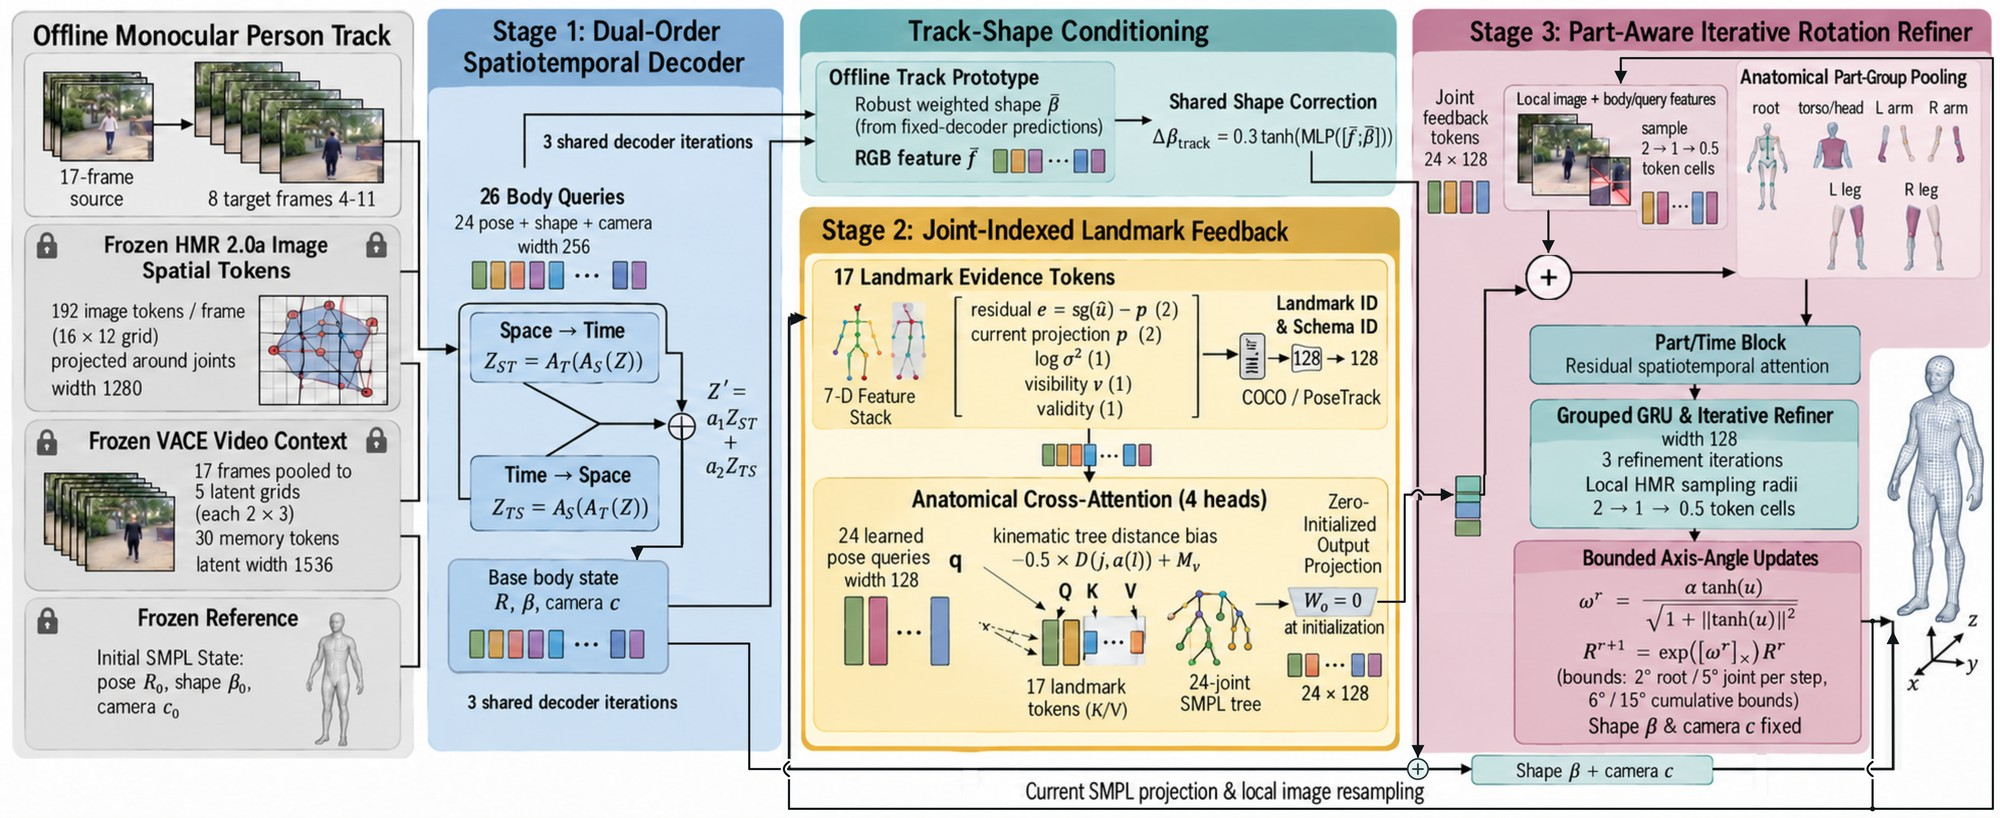
\includegraphics[width=\textwidth]{figures/overview_final.jpg}
  \caption{\textbf{\method overview.}
  A frozen dual-order spatiotemporal decoder reads HMR\,2.0a image tokens and Wan/VACE video context and predicts a residual to a frozen reference body; a track-conditioned residual shares shape over a person track.
  The final stage refines rotations for three iterations: landmark evidence is routed to 24 joint queries, added before part pooling and masked temporal exchange, and converted into bounded axis-angle updates; projections and local image samples are recomputed at every iteration.
  \TODO{Redraw stage~2 for C11: evidence tokens come from an external detector (residual $u{-}p$, projection $p$, $-2\log c$, $c$, validity) instead of the inherited head; the drawn step bounds $2^\circ/5^\circ$ are the scales $\alpha$, the tight cumulative bounds are $5.2^\circ/13.0^\circ$ (\cref{sec:refiner}).}}
  \label{fig:overview}
\end{figure*}

\section{Method}
\label{sec:method}

\subsection{Setting and inherited model}
\label{sec:setting}

Given an offline monocular person track, \method predicts for every target frame $t$ a camera-space SMPL state $x_t=(R_t,\beta_t,c_t)$ with 24 joint rotations, ten shape coefficients and a crop camera $c_t=(s_t,t_{x,t},t_{y,t})$.
All variants in this paper share one trained \emph{parent}, which we keep fixed and describe only briefly.
Each eight-frame target window reads 192 HMR\,2.0a tokens per frame~\cite{goel2023hmr2} and a 17-frame Wan/VACE context~\cite{wan2025wan,jiang2025vace} compressed to 30 memory tokens; both encoders are frozen, and the video-generation models Wan and VACE serve only as feature extractors.
Twenty-six body queries $Z$ (24 pose, shape, camera) are decoded by blocks that mix a spatial-first order $Z_{\mathrm{ST}}=A_T(A_S(Z))$ and a temporal-first order $Z_{\mathrm{TS}}=A_S(A_T(Z))$ of attention,
\begin{equation}
  Z' = a_1 Z_{\mathrm{ST}} + a_2 Z_{\mathrm{TS}},\qquad a=\softmax\big(g([Z_{\mathrm{ST}};Z_{\mathrm{TS}}])\big),
  \label{eq:dual}
\end{equation}
over three weight-shared iterations that predict a residual to a frozen reference body, using the continuous 6D rotation representation~\cite{zhou2019continuity}.
A track-conditioned residual, bounded componentwise by 0.3, maps a fixed prediction-and-image prototype of the track to a shape correction shared by all of its frames.
The final stage, a part-aware recurrent rotation refiner (\cref{sec:refiner}), is where landmark evidence enters; only its feedback module differs between variants.

\subsection{What did joint-indexed feedback route?}
\label{sec:audit}

This earlier variant, denoted C10, read 17 landmark observations $\hat u_{tl}$ from an observation head of the parent, together with a log-variance and a visibility logit, and formed the residual $\sg(\hat u_{tl})-p_{tl}(x^r)$ to the current projection $p_{tl}(x^r)$.
Every 2D loss weight was zero in all stages that produced the parent and C10, so the head never received gradient.
Its coordinate layers remain at their zero initialisation, which makes $\hat u_{tl}$ the projection of the frozen reference body; the log-variance stays at its bias of $-4$ and the visibility at $\sigma(0)=0.5$.
The routed residual is therefore $p_{tl}(x^{\text{ref}})-p_{tl}(x^r)$: the image-plane drift of the current body from the reference, with constant uncertainty features.
\TODO{confirm on the archived parent, C00 and C10 checkpoints with scripts/inspect\_checkpoint\_v43.py; report the measured verdict (all coordinate weights exactly zero, log-variance bias $-4$) here and in Supp.~S5.}
Such a signal can still help a refiner, for instance as a learned pull towards the reference, but it contains no image evidence, so an advantage of routing it cannot be attributed to evidence assignment.
Two further limitations affect the archived comparison: the mean-feedback control (C00) mapped four averaged scalars through 512 parameters, against 105,472 for the router, and both runs used a single seed with validation-only evaluation.
Relative to its parent, archived C10 changed validation MPJPE by $-0.07$\,mm with a sequence-bootstrap 95\% interval of $[-0.21, +0.03]$ (Supp.~S5).
We keep this self-referential router as variant \vA{2} and its mean control as \vA{1}, and build the method below on external evidence.

\begin{figure*}[t]
  \centering
  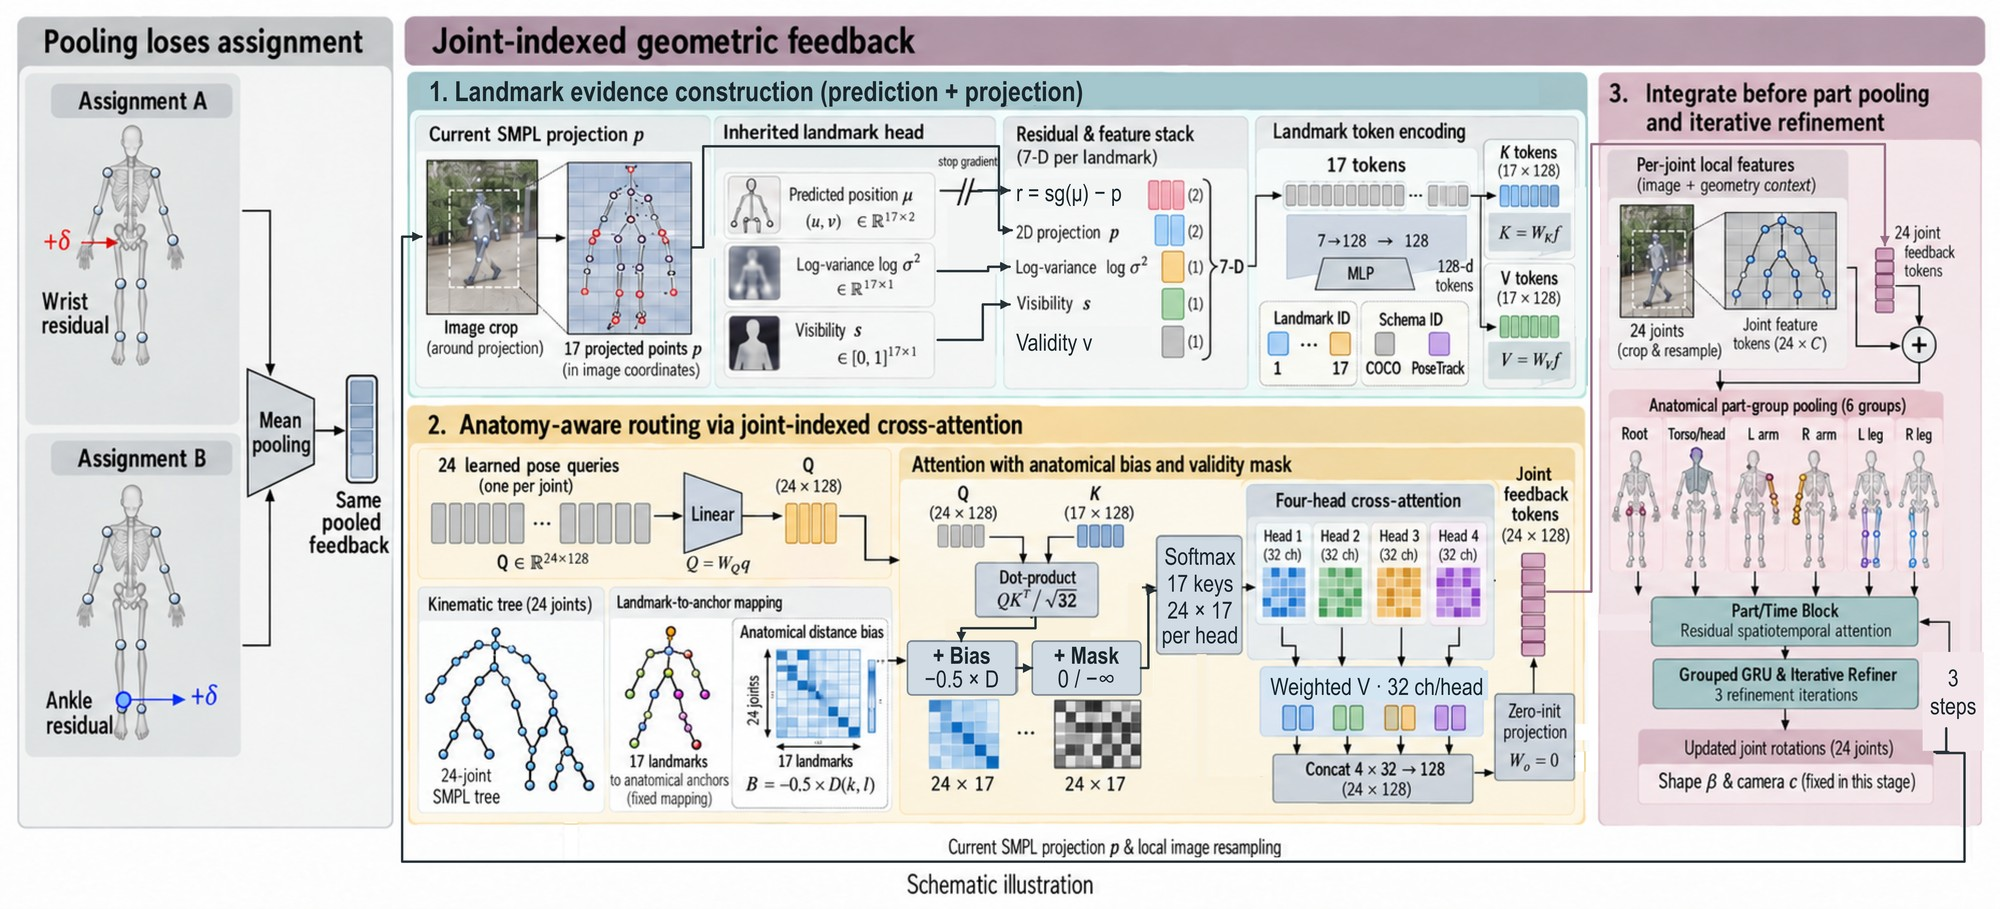
\includegraphics[width=0.88\textwidth]{figures/identity_final.jpg}
  \caption{\textbf{Identity-preserving routing} (schematic).
  Left: exchanging a wrist and an ankle residual leaves a mean-pooled feedback vector unchanged.
  Right: every landmark becomes a token with identity and schema embeddings; 24 joint queries read the 17 tokens through four-head attention with the kinematic-tree bias $-D/2$ and a validity mask, and the zero-initialised output is added to each joint before part pooling and the recurrent update.
  \TODO{Redraw panel~1 for C11: the evidence comes from an external detector (ViTPose keypoints $u$ and confidences $c$) instead of the inherited landmark head.}}
  \label{fig:identity}
\end{figure*}

\subsection{Identity-bearing evidence tokens}
\label{sec:tokens}

An external top-down detector, ViTPose~\cite{xu2022vitpose,xu2024vitposepp} (ViTPose++-H, COCO-17 expert), runs on the same $256\times256$ crop as the image backbone and returns, for each landmark $l\in\{1,\dots,17\}$, a position $u_{tl}$ in normalised crop coordinates and a confidence $c_{tl}\in[0,1]$.
Let $p_{tl}(x^r)$ be the COCO landmark regressed from the current SMPL mesh at refinement iteration $r$ and projected with the crop camera.
Each landmark becomes a seven-dimensional feature
\begin{equation}
  \phi^r_{tl} = \big[\,u_{tl}-p_{tl}(x^r);\; p_{tl}(x^r);\; -2\log c_{tl};\; c_{tl};\; v_{tl}\,\big],
  \label{eq:token}
\end{equation}
where $v_{tl}$ marks finite keypoints with positive confidence in valid frames, invalid entries are zeroed, and residual, projection and log-confidence are clipped to $[-2,2]$, $[-4,4]$ and $[-6,6]$.
The term $-2\log c$ plays the role of a log-variance and vanishes for confident detections.
A two-layer MLP maps $\phi^r_{tl}$ to width 128, and a learned landmark embedding $e_l$ plus a schema embedding are added, so that the token $z^r_{tl}$ carries its anatomical identity independently of its content.
Because $p_{tl}(x^r)$ is recomputed from the current body, the residual shrinks or changes direction as the refiner moves the joints; the evidence is a closed-loop signal rather than a fixed input.

\subsection{Anatomically biased routing}
\label{sec:routing}

Twenty-four learned joint queries $q_j$ read the evidence tokens of a person-frame with four-head attention (\cref{fig:identity}),
\begin{equation}
  A^h_{jl} = \softmax_l\!\Big(\frac{(W^h_Q q_j)^{\!\top} W^h_K z^r_{tl}}{\sqrt{d_h}} - \frac{D(j,a(l))}{2} + M_{tl}\Big),
  \label{eq:route}
\end{equation}
with $d_h=32$, where $a(l)$ is the anatomical anchor of landmark $l$ (the head joint for facial landmarks and the corresponding SMPL joint for limb landmarks), $D$ the shortest-path distance on the SMPL kinematic tree and $M_{tl}\in\{0,-\infty\}$ the validity mask.
The bias favours nearby anatomy without forbidding long-range reads, \eg a wrist query may still consult the shoulder.
The attention-weighted values of the four heads are concatenated, projected, and mapped by a final matrix $W_o$ to 24 joint feedback vectors $f^r_{tj}\in\mathbb{R}^{128}$.
We initialise $W_o=0$, so the feedback is exactly zero at the start of training while $W_o$ receives gradient immediately; together with zero-initialised residual blocks, every variant reproduces the parent's predictions before its first update.
A frame without any valid landmark receives zero feedback.
The router trains 105,472 parameters, as many as C10.
For fusion with the inherited head (\vB{6}), the 17 head tokens and the 17 external tokens, each with their own identity embeddings and anchors, form one set of 34 tokens.

\paragraph{Controls as single-factor changes.}
Every control keeps the token features of \cref{eq:token} and the zero-initialised output, and changes one factor (\cref{tab:main,tab:ablation}).
The \emph{pooled} control (\vB{1}) removes identity and routing: the per-token MLP outputs are averaged over valid landmarks, as in Deep Sets~\cite{zaheer2017deepsets}, passed through a 128--256--128 MLP and broadcast to all joints (100,096 parameters).
The \emph{ordered-vector} control (\vB{7}) keeps identity by position: the 17 encoded tokens are concatenated in slot order, mapped by a linear layer and an MLP, and broadcast to all joints, mirroring how keypoints condition WHAM-style models (329,344 parameters, $3.1\times$ the router).
The \emph{set} control (\vB{2}) keeps the joint queries but removes identity embeddings and bias, which yields Set-Transformer-style pooling by attention~\cite{lee2019settransformer} that is invariant to permuting landmarks.
\vB{3} keeps identity but removes the bias, and \vB{5} keeps identity with a bias whose landmark columns are permuted by a fixed derangement, \ie a wrong anatomy with identical bias statistics.
Note that the projected coordinates $p_{tl}$ may reveal identity implicitly even when embeddings are removed; \vB{1} and \vB{2} therefore test whether \emph{explicit} identity and routing help at this budget, not whether identity is recoverable in principle.

\subsection{Part-aware iterative rotation refinement}
\label{sec:refiner}

At iteration $r$, each joint feature combines its contextual pose query, the current body state and local HMR\,2.0a samples around its projection, whose radius shrinks from two to one to half a token cell.
The routed feedback $f^r_{tj}$ is added to this per-joint feature \emph{before} the joints are pooled into six anatomical groups (root, torso/head, two arms, two legs).
Two residual blocks then exchange information across groups within a frame and across time within a group; temporal attention is masked by source-frame identities so that duplicated or invalid frames and track gaps never act as independent evidence.
The group context is broadcast back to the joints, and a group-specific GRU, whose state persists over the three refinement iterations rather than over video frames, predicts $u^r_{tj}\in\mathbb{R}^3$, converted to a bounded axis-angle increment,
\begin{equation}
  \omega^r_{tj} = \alpha_j\,\frac{\tanh u^r_{tj}}{\sqrt{1+\lVert\tanh u^r_{tj}\rVert^2}},\qquad R^{r+1}_{tj} = \exp([\omega^r_{tj}]_\times)\,R^r_{tj},
  \label{eq:bound}
\end{equation}
with $\tanh$ applied componentwise and $\alpha_j=2^\circ$ for the root and $5^\circ$ otherwise.
Since $\lVert\tanh u\rVert<\sqrt3$ and $s/\sqrt{1+s^2}$ is increasing, each increment is smaller than $\tfrac{\sqrt3}{2}\alpha_j$, \ie $1.73^\circ$ for the root and $4.33^\circ$ for other joints, and the triangle inequality on rotations bounds the displacement after three iterations by $5.2^\circ$ and $13.0^\circ$ relative to the refiner input.
Shape and camera pass through unchanged, while projections, local samples and the routed evidence are recomputed after every update.

\paragraph{Objective.}
All variants use one objective: joint and vertex errors in metres, rotation and shape supervision, velocity and acceleration of the hip-centred prediction-minus-target joint error, a Procrustes-aligned joint auxiliary, intermediate decoder supervision and small consistency and update penalties (coefficients in Supp.~S2).
Every person-frame is owned by one window, and acceleration triplets that straddle window boundaries are retained by forwarding their owner contexts, so the motion objective and metric cover complete sequences.
No 2D reprojection loss is used; external keypoints act only as inputs.

\section{Experiments}
\label{sec:experiments}

\subsection{Protocol}
\label{sec:protocol}

\paragraph{Data.}
We use 3DPW~\cite{vonmarcard2018pw3d} with its official splits.
The refiner trains on the training split (2,909 eight-frame windows, 22,735 person-frames); every model is evaluated on validation (12 sequences, 10,413 person-frames, 10,226 acceleration triplets) and, once, on test (24 sequences, 35,515 person-frames, 34,752 triplets).
A test evaluation is only accepted through an immutable lock that binds the checkpoint hash, configuration, weight type and complete validation result.
Person crops follow the dataset's 2D person annotations with a 25\% margin, and track identities come from the annotations; Supp.~S3 lists these and other deviations from detector-and-tracker pipelines.
Earlier models of this project were evaluated on the test split before this study; no decision reported here used test results, but that exposure cannot be undone.

\paragraph{Metrics.}
MPJPE uses the 14 LSP joints regressed with the H36M regressor; PA-MPJPE additionally applies a per-frame similarity Procrustes alignment.
Root conventions differ across the literature, so we report MPJPE and PVE both relative to the H36M pelvis (joint~0; SPIN, CameraHMR, ReFit, PromptHMR) and relative to the hip midpoint (VIBE evaluator, WHAM, GVHMR), and compare each published row only under its own convention.
Controlled tables use the pelvis root; our historical unaligned PVE is kept in the supplement.
Acceleration error (Accel) is the second difference of the hip-centred prediction-minus-target joint error over all annotation-adjacent triplets, including triplets across inference windows, in mm/frame$^2$; multiplied by $0.9$ it gives m/s$^2$ at 30\,fps, the unit used by WHAM and GVHMR.
We apply no flip averaging and no temporal smoothing.

\paragraph{Training and selection.}
Every variant starts from the same parent and trains for 1,000 steps with identical data order, losses and staged unfreezing (AdamW, effective batch of 16 windows; Supp.~S2), with seeds 2026, 2027 and 2028; the router initialisation seed follows the training seed.
We evaluate the EMA weights at step 1,000 for every variant and seed, a choice fixed before training; no variant, step or seed is selected on validation or test.
The archived parent (\textsf{P}), C10 and C00 checkpoints are evaluated with the same code path.

\paragraph{Statistics.}
We report the mean and standard deviation over seeds.
A paired comparison gives the difference $\Delta$ of the frame-weighted aggregate error, averaged over the paired seeds (negative favours the first variant), and a 95\% percentile interval from a hierarchical cluster bootstrap~\cite{efron1993bootstrap} that resamples seeds and then sequences (20,000 resamples), because frames within a sequence are strongly correlated.
We also count the sequences whose seed-averaged error decreases; paired $t$-tests over seeds are listed in the supplement but have little power with three seeds.
The comparisons in \cref{tab:paired} and the rule that a difference is reliable only if its interval excludes zero and all three seeds agree in sign were fixed before any test evaluation.

\begin{table*}[t]
  \centering
  \footnotesize
  \setlength{\tabcolsep}{4pt}
  \begin{tabular}{@{}l l c c c c c c@{}}
    \toprule
    Method & Input; setting & 3DPW train & Root & MPJPE$\downarrow$ & PA-MPJPE$\downarrow$ & PVE$\downarrow$ & Accel$\downarrow$ \\
    \midrule
    \multicolumn{8}{@{}l}{\emph{Author-reported 3DPW test results}}\\
    PyMAF~\cite{zhang2021pymaf}         & Image; ResNet-50          & No  & --  & 92.8 & 58.9 & 110.1$^\ast$ & -- \\
    PARE~\cite{kocabas2021pare}         & Image; HRNet-W32          & No  & --  & 82.0 & 50.9 & 97.9$^\ast$  & -- \\
    PARE~\cite{kocabas2021pare}         & Image; HRNet-W32          & Yes & --  & 74.5 & 46.5 & 88.6$^\ast$  & -- \\
    CLIFF~\cite{li2022cliff}            & Image; HRNet-W48          & Yes & P   & 69.0 & 43.0 & 81.2$^\ast$ & -- \\
    PyMAF-X~\cite{zhang2023pymafx}      & Image; body-only HR48     & No  & P   & 78.0 & 47.1 & 91.3$^\ast$ & -- \\
    PyMAF-X~\cite{zhang2023pymafx}      & Image; body-only HR48     & Yes & P   & 74.2 & 45.3 & 87.0$^\ast$ & -- \\
    HMR\,2.0a~\cite{goel2023hmr2}       & Image; ViT                & No  & --  & 70.0 & 44.5 & --    & -- \\
    HMR\,2.0b~\cite{goel2023hmr2}       & Image; ViT                & No  & --  & 81.3 & 54.3 & --    & -- \\
    ReFit~\cite{wang2023refit}          & Image; HRNet              & Yes & P   & 65.8 & 41.0 & --    & -- \\
    ReFit~\cite{wang2023refit}          & Image; BEDLAM + real      & Yes & P   & 57.6 & 38.2 & 67.6  & -- \\
    CameraHMR~\cite{patel2025camerahmr} & Image; all data + 3DPW    & Yes & P   & 56.0 & 35.1 & 65.9  & -- \\
    PromptHMR~\cite{wang2025prompthmr}  & Image; GT focal length    & Yes & P   & 58.7 & 36.6 & 69.4  & -- \\
    VIBE~\cite{kocabas2020vibe}         & Video; SPIN features      & Yes & H   & 82.9 & 51.9 & 99.1$^\ddagger$  & 23.4$^\dagger$ \\
    TCMR~\cite{choi2021tcmr}            & Video; temporal context   & Yes & H   & 86.5 & 52.7 & 102.9$^\ddagger$ & 7.1$^\dagger$ \\
    GLoT~\cite{shen2023glot}            & Video; 16 frames          & Yes & H   & 80.7 & 50.6 & 96.3$^\ddagger$  & 6.6$^\dagger$ \\
    WHAM~\cite{shin2024wham}            & Video; ViT; real data     & Yes & H   & 57.8 & 35.9 & 68.7  & 6.6 \\
    WHAM~\cite{shin2024wham}            & Video; ViT; + BEDLAM      & Yes & H   & 56.9 & 35.7 & 67.4  & 6.7 \\
    GVHMR~\cite{shen2024gvhmr}          & Video; flip evaluation    & Yes & H   & 55.6 & 36.2 & 67.2  & 5.0 \\
    PromptHMR~\cite{wang2025prompthmr}  & Video; no flip averaging  & Yes & P   & 56.9 & 35.5 & 67.3  & -- \\
    OnlineHMR~\cite{zhao2026onlinehmr}  & Causal online video       & Yes & --  & 69.9 & 43.7 & 83.7$^\ast$  & -- \\
    \midrule
    \multicolumn{8}{@{}l}{\emph{Ours, 3DPW test, annotation-derived crops, no flip or smoothing; root P\,/\,H}}\\
    Parent \textsf{P}            & Video; HMR\,2.0a + VACE   & Yes & P\,/\,H & \res{P-parent@test@mpjpe}\,/\,\res{P-parent@test@mpjpehip} & \res{P-parent@test@pampjpe} & \res{P-parent@test@pvepelvis}\,/\,\res{P-parent@test@pvehip} & \res{P-parent@test@accelms} \\
    C10 (archived, routes drift) & + head routing            & Yes & P\,/\,H & \res{R-c10-archived@test@mpjpe}\,/\,\res{R-c10-archived@test@mpjpehip} & \res{R-c10-archived@test@pampjpe} & \res{R-c10-archived@test@pvepelvis}\,/\,\res{R-c10-archived@test@pvehip} & \res{R-c10-archived@test@accelms} \\
    \vA{1} mean (C00 design)     & + head mean               & Yes & P\,/\,H & \res{A1-mean@test@mpjpe}\,/\,\res{A1-mean@test@mpjpehip} & \res{A1-mean@test@pampjpe} & \res{A1-mean@test@pvepelvis}\,/\,\res{A1-mean@test@pvehip} & \res{A1-mean@test@accelms} \\
    \vB{7} ordered vector        & + ViTPose, concatenated   & Yes & P\,/\,H & \res{B7-ext-concat@test@mpjpe}\,/\,\res{B7-ext-concat@test@mpjpehip} & \res{B7-ext-concat@test@pampjpe} & \res{B7-ext-concat@test@pvepelvis}\,/\,\res{B7-ext-concat@test@pvehip} & \res{B7-ext-concat@test@accelms} \\
    \vB{4} \method (routed)      & + ViTPose, routed         & Yes & P\,/\,H & \res{B4-ext-joint@test@mpjpe}\,/\,\res{B4-ext-joint@test@mpjpehip} & \res{B4-ext-joint@test@pampjpe} & \res{B4-ext-joint@test@pvepelvis}\,/\,\res{B4-ext-joint@test@pvehip} & \res{B4-ext-joint@test@accelms} \\
    \vB{6} head + ViTPose        & + both, routed            & Yes & P\,/\,H & \res{B6-both-joint@test@mpjpe}\,/\,\res{B6-both-joint@test@mpjpehip} & \res{B6-both-joint@test@pampjpe} & \res{B6-both-joint@test@pvepelvis}\,/\,\res{B6-both-joint@test@pvehip} & \res{B6-both-joint@test@accelms} \\
    \bottomrule
  \end{tabular}
  \caption{\textbf{3DPW test results} (mm; Accel in m/s$^2$).
  Published rows are the authors' own numbers with their inputs and training data.
  Root gives the convention under which MPJPE and PVE were computed: P, vertices and joints relative to the H36M-regressed pelvis; H, relative to the hip midpoint; --, not reported, or convention or unit not established by our audit of the source.
  Our rows give both conventions (P\,/\,H) and are means over three seeds (single checkpoints for \textsf{P} and C10); compare each published row only with the matching value.
  $^\ast$PVE alignment not audited.
  $^\ddagger$Unaligned PVE against neutral-gender ground-truth bodies, which our evaluator does not reproduce; not comparable.
  $^\dagger$Frame-based acceleration as printed (mm/frame$^2$, not converted).
  Our crops are derived from dataset annotations, so these rows are not a like-for-like ranking (\cref{sec:protocol}).}
  \label{tab:sota}
\end{table*}

\subsection{Comparison with published results}
\label{sec:sota}

\Cref{tab:sota} places our test results next to author-reported numbers, keeping strong variants with additional training data and recording each row's input, training data and evaluation convention.
\TODO{Describe where \vB{4} falls relative to the hip-root video methods (WHAM, GVHMR) and the pelvis-root image methods (CameraHMR, ReFit, PromptHMR) using the matching column only; do not claim state of the art, and recall the annotation-derived crops.}
Temporal quality is a clear weakness of our refiner.
The archived C10 checkpoint has an acceleration error of 21.44\,mm/frame$^2$ on validation (archived, single seed), \ie 19.3\,m/s$^2$, whereas WHAM and GVHMR report 6.6 and 5.0\,m/s$^2$ on test.
Our refiner applies no temporal smoothing and is not a motion prior: temporal attention exchanges features between frames, and the acceleration term is one loss among several over a short continuation.
\TODO{Confirm with \res{B4-ext-joint@test@accelms}\,m/s$^2$ and state whether routing changes temporal error (\cref{tab:paired}, Accel column).}

\begin{table*}[t]
  \centering
  \footnotesize
  \setlength{\tabcolsep}{3.2pt}
  \begin{tabular}{@{}l l l r cccc cccc@{}}
    \toprule
    & & & & \multicolumn{4}{c}{Validation} & \multicolumn{4}{c}{Test} \\
    \cmidrule(lr){5-8}\cmidrule(l){9-12}
    ID & Evidence & Interface & Params & MPJPE & PA-MPJPE & PVE & Accel & MPJPE & PA-MPJPE & PVE & Accel \\
    \midrule
    \textsf{P} & \multicolumn{2}{l}{parent, no continuation} & -- &
      \res{P-parent@validation@mpjpe} & \res{P-parent@validation@pampjpe} & \res{P-parent@validation@pvepelvis} & \res{P-parent@validation@accel} &
      \res{P-parent@test@mpjpe} & \res{P-parent@test@pampjpe} & \res{P-parent@test@pvepelvis} & \res{P-parent@test@accel} \\
    \midrule
    \vA{0} & none & -- & 0 &
      \res{A0-none@validation@mpjpe@pm} & \res{A0-none@validation@pampjpe@pm} & \res{A0-none@validation@pvepelvis@pm} & \res{A0-none@validation@accel@pm} &
      \res{A0-none@test@mpjpe@pm} & \res{A0-none@test@pampjpe@pm} & \res{A0-none@test@pvepelvis@pm} & \res{A0-none@test@accel@pm} \\
    \vA{1} & head (drift) & mean (C00) & 512 &
      \res{A1-mean@validation@mpjpe@pm} & \res{A1-mean@validation@pampjpe@pm} & \res{A1-mean@validation@pvepelvis@pm} & \res{A1-mean@validation@accel@pm} &
      \res{A1-mean@test@mpjpe@pm} & \res{A1-mean@test@pampjpe@pm} & \res{A1-mean@test@pvepelvis@pm} & \res{A1-mean@test@accel@pm} \\
    \vA{2} & head (drift) & routed (C10) & 105,472 &
      \res{A2-head-joint@validation@mpjpe@pm} & \res{A2-head-joint@validation@pampjpe@pm} & \res{A2-head-joint@validation@pvepelvis@pm} & \res{A2-head-joint@validation@accel@pm} &
      \res{A2-head-joint@test@mpjpe@pm} & \res{A2-head-joint@test@pampjpe@pm} & \res{A2-head-joint@test@pvepelvis@pm} & \res{A2-head-joint@test@accel@pm} \\
    \vB{1} & ViTPose & pooled & 100,096 &
      \res{B1-ext-pooled@validation@mpjpe@pm} & \res{B1-ext-pooled@validation@pampjpe@pm} & \res{B1-ext-pooled@validation@pvepelvis@pm} & \res{B1-ext-pooled@validation@accel@pm} &
      \res{B1-ext-pooled@test@mpjpe@pm} & \res{B1-ext-pooled@test@pampjpe@pm} & \res{B1-ext-pooled@test@pvepelvis@pm} & \res{B1-ext-pooled@test@accel@pm} \\
    \vB{7} & ViTPose & ordered vector & 329,344 &
      \res{B7-ext-concat@validation@mpjpe@pm} & \res{B7-ext-concat@validation@pampjpe@pm} & \res{B7-ext-concat@validation@pvepelvis@pm} & \res{B7-ext-concat@validation@accel@pm} &
      \res{B7-ext-concat@test@mpjpe@pm} & \res{B7-ext-concat@test@pampjpe@pm} & \res{B7-ext-concat@test@pvepelvis@pm} & \res{B7-ext-concat@test@accel@pm} \\
    \vB{4} & ViTPose & routed (ours) & 105,472 &
      \res{B4-ext-joint@validation@mpjpe@pm} & \res{B4-ext-joint@validation@pampjpe@pm} & \res{B4-ext-joint@validation@pvepelvis@pm} & \res{B4-ext-joint@validation@accel@pm} &
      \res{B4-ext-joint@test@mpjpe@pm} & \res{B4-ext-joint@test@pampjpe@pm} & \res{B4-ext-joint@test@pvepelvis@pm} & \res{B4-ext-joint@test@accel@pm} \\
    \bottomrule
  \end{tabular}
  \caption{\textbf{Controlled comparison} on 3DPW (mean{\scriptsize$\pm$std} over three seeds; mm, Accel in mm/frame$^2$; pelvis root, pelvis-aligned PVE).
  All variants continue the same parent \textsf{P} for 1,000 steps and are evaluated with EMA weights at that pre-registered step.
  ``Head (drift)'' denotes the inherited observation head, whose outputs equal the frozen reference projection (\cref{sec:audit}).
  Params counts the feedback module parameters that receive gradient.
  Archived single-seed validation values for reference: parent 61.26/37.64/73.02, C10 61.19/37.61/72.82, C00 61.26/37.64/73.05\,mm (MPJPE/PA-MPJPE/unaligned PVE; C00 transcribed from run records).}
  \label{tab:main}
\end{table*}

\subsection{Does real evidence help, and through which interface?}
\label{sec:main}

\Cref{tab:main} reports the core variants and \cref{tab:paired} their paired differences on test.
Continuing the parent without any landmark channel (\vA{0}) isolates the effect of the extra budget: \vA{0} reaches \res{A0-none@test@mpjpe}\,mm test MPJPE, against \res{P-parent@test@mpjpe}\,mm for the parent.

\paragraph{Self-referential evidence.}
Mean (\vA{1}) and routed (\vA{2}) head feedback re-run the archived C00/C10 designs with three seeds.
Against no feedback, routed drift gives \dtext{A2-head-joint}{A0-none}{test}{mpjpe}, and routed against mean drift gives \dtext{A2-head-joint}{A1-mean}{test}{mpjpe}.
\TODO{If both CIs include 0: state that the archived C10 advantage does not survive three seeds and the test split, consistent with routing a signal that contains no image evidence. If A2 beats A0: discuss the reference-drift signal as a learned pull toward the reference (regulariser), not evidence.}

\paragraph{External evidence.}
Routing ViTPose evidence instead of drift changes test MPJPE by \dtext{B4-ext-joint}{A2-head-joint}{test}{mpjpe}, and relative to no feedback by \dtext{B4-ext-joint}{A0-none}{test}{mpjpe}.
\TODO{State whether real evidence helps (CI of B4 vs A0 excludes 0) and by how much on PVE (\cref{tab:paired}).}

\paragraph{Identity and routing.}
The central comparison holds the evidence fixed and changes only the interface.
Against the capacity-matched pooled control, routing gives \dtext{B4-ext-joint}{B1-ext-pooled}{test}{mpjpe}; against ordered-vector conditioning, which keeps identity by position with $3.1\times$ more parameters, it gives \dtext{B4-ext-joint}{B7-ext-concat}{test}{mpjpe}.
\TODO{Decision rule (reliable = CI excludes 0 and all seeds agree in sign). B4 better than both B1 and B7: anatomically routed tokens beat pooled and ordered-vector (WHAM-style) conditioning at equal evidence. B4 $\approx$ B7, both better than B1: identity matters but routing is not required; argue parameter efficiency (105k \vs 329k), interpretability and multi-source fusion (B6). B4 $\approx$ B1 $\approx$ A0: external evidence does not help this refiner; reframe the paper around the self-referential-evidence diagnostic and the controlled protocol.}

\begin{table*}[t]
  \centering
  \footnotesize
  \setlength{\tabcolsep}{4pt}
  \begin{tabular}{@{}l l c c c c c c@{}}
    \toprule
    Comparison & Isolated factor & $\Delta$MPJPE [95\% CI] & Wins & $\Delta$PVE [95\% CI] & Wins & $\Delta$PA-MPJPE & $\Delta$Accel \\
    \midrule
    \vB{4} \vs \vB{1} & routing \vs capacity-matched pooling & \dci{B4-ext-joint}{B1-ext-pooled}{test}{mpjpe} & \cmpwins{B4-ext-joint}{B1-ext-pooled}{test}{mpjpe} & \dci{B4-ext-joint}{B1-ext-pooled}{test}{pvepelvis} & \cmpwins{B4-ext-joint}{B1-ext-pooled}{test}{pvepelvis} & \cmpdiff{B4-ext-joint}{B1-ext-pooled}{test}{pampjpe} & \cmpdiff{B4-ext-joint}{B1-ext-pooled}{test}{accel} \\
    \vB{4} \vs \vB{7} & routing \vs ordered vector & \dci{B4-ext-joint}{B7-ext-concat}{test}{mpjpe} & \cmpwins{B4-ext-joint}{B7-ext-concat}{test}{mpjpe} & \dci{B4-ext-joint}{B7-ext-concat}{test}{pvepelvis} & \cmpwins{B4-ext-joint}{B7-ext-concat}{test}{pvepelvis} & \cmpdiff{B4-ext-joint}{B7-ext-concat}{test}{pampjpe} & \cmpdiff{B4-ext-joint}{B7-ext-concat}{test}{accel} \\
    \vB{4} \vs \vB{2} & explicit identity + bias & \dci{B4-ext-joint}{B2-ext-set}{test}{mpjpe} & \cmpwins{B4-ext-joint}{B2-ext-set}{test}{mpjpe} & \dci{B4-ext-joint}{B2-ext-set}{test}{pvepelvis} & \cmpwins{B4-ext-joint}{B2-ext-set}{test}{pvepelvis} & \cmpdiff{B4-ext-joint}{B2-ext-set}{test}{pampjpe} & \cmpdiff{B4-ext-joint}{B2-ext-set}{test}{accel} \\
    \vB{4} \vs \vB{3} & anatomical bias & \dci{B4-ext-joint}{B3-ext-nobias}{test}{mpjpe} & \cmpwins{B4-ext-joint}{B3-ext-nobias}{test}{mpjpe} & \dci{B4-ext-joint}{B3-ext-nobias}{test}{pvepelvis} & \cmpwins{B4-ext-joint}{B3-ext-nobias}{test}{pvepelvis} & \cmpdiff{B4-ext-joint}{B3-ext-nobias}{test}{pampjpe} & \cmpdiff{B4-ext-joint}{B3-ext-nobias}{test}{accel} \\
    \vB{4} \vs \vB{5} & correct \vs deranged anatomy & \dci{B4-ext-joint}{B5-ext-shuffled}{test}{mpjpe} & \cmpwins{B4-ext-joint}{B5-ext-shuffled}{test}{mpjpe} & \dci{B4-ext-joint}{B5-ext-shuffled}{test}{pvepelvis} & \cmpwins{B4-ext-joint}{B5-ext-shuffled}{test}{pvepelvis} & \cmpdiff{B4-ext-joint}{B5-ext-shuffled}{test}{pampjpe} & \cmpdiff{B4-ext-joint}{B5-ext-shuffled}{test}{accel} \\
    \vB{4} \vs \vA{2} & external \vs self-referential evidence & \dci{B4-ext-joint}{A2-head-joint}{test}{mpjpe} & \cmpwins{B4-ext-joint}{A2-head-joint}{test}{mpjpe} & \dci{B4-ext-joint}{A2-head-joint}{test}{pvepelvis} & \cmpwins{B4-ext-joint}{A2-head-joint}{test}{pvepelvis} & \cmpdiff{B4-ext-joint}{A2-head-joint}{test}{pampjpe} & \cmpdiff{B4-ext-joint}{A2-head-joint}{test}{accel} \\
    \vB{6} \vs \vB{4} & adding head tokens & \dci{B6-both-joint}{B4-ext-joint}{test}{mpjpe} & \cmpwins{B6-both-joint}{B4-ext-joint}{test}{mpjpe} & \dci{B6-both-joint}{B4-ext-joint}{test}{pvepelvis} & \cmpwins{B6-both-joint}{B4-ext-joint}{test}{pvepelvis} & \cmpdiff{B6-both-joint}{B4-ext-joint}{test}{pampjpe} & \cmpdiff{B6-both-joint}{B4-ext-joint}{test}{accel} \\
    \vB{1} \vs \vA{1} & external \vs drift, pooled & \dci{B1-ext-pooled}{A1-mean}{test}{mpjpe} & \cmpwins{B1-ext-pooled}{A1-mean}{test}{mpjpe} & \dci{B1-ext-pooled}{A1-mean}{test}{pvepelvis} & \cmpwins{B1-ext-pooled}{A1-mean}{test}{pvepelvis} & \cmpdiff{B1-ext-pooled}{A1-mean}{test}{pampjpe} & \cmpdiff{B1-ext-pooled}{A1-mean}{test}{accel} \\
    \vA{2} \vs \vA{1} & routed \vs mean drift (C10 \vs C00) & \dci{A2-head-joint}{A1-mean}{test}{mpjpe} & \cmpwins{A2-head-joint}{A1-mean}{test}{mpjpe} & \dci{A2-head-joint}{A1-mean}{test}{pvepelvis} & \cmpwins{A2-head-joint}{A1-mean}{test}{pvepelvis} & \cmpdiff{A2-head-joint}{A1-mean}{test}{pampjpe} & \cmpdiff{A2-head-joint}{A1-mean}{test}{accel} \\
    \vA{1} \vs \vA{0} & mean drift \vs none & \dci{A1-mean}{A0-none}{test}{mpjpe} & \cmpwins{A1-mean}{A0-none}{test}{mpjpe} & \dci{A1-mean}{A0-none}{test}{pvepelvis} & \cmpwins{A1-mean}{A0-none}{test}{pvepelvis} & \cmpdiff{A1-mean}{A0-none}{test}{pampjpe} & \cmpdiff{A1-mean}{A0-none}{test}{accel} \\
    \vA{2} \vs \vA{0} & routed drift \vs none & \dci{A2-head-joint}{A0-none}{test}{mpjpe} & \cmpwins{A2-head-joint}{A0-none}{test}{mpjpe} & \dci{A2-head-joint}{A0-none}{test}{pvepelvis} & \cmpwins{A2-head-joint}{A0-none}{test}{pvepelvis} & \cmpdiff{A2-head-joint}{A0-none}{test}{pampjpe} & \cmpdiff{A2-head-joint}{A0-none}{test}{accel} \\
    \vB{4} \vs \vA{0} & routed evidence \vs none & \dci{B4-ext-joint}{A0-none}{test}{mpjpe} & \cmpwins{B4-ext-joint}{A0-none}{test}{mpjpe} & \dci{B4-ext-joint}{A0-none}{test}{pvepelvis} & \cmpwins{B4-ext-joint}{A0-none}{test}{pvepelvis} & \cmpdiff{B4-ext-joint}{A0-none}{test}{pampjpe} & \cmpdiff{B4-ext-joint}{A0-none}{test}{accel} \\
    \vC{4} \vs \vC{1} & routing \vs pooling, OpenPose & \dci{C4-op-joint}{C1-op-pooled}{test}{mpjpe} & \cmpwins{C4-op-joint}{C1-op-pooled}{test}{mpjpe} & \dci{C4-op-joint}{C1-op-pooled}{test}{pvepelvis} & \cmpwins{C4-op-joint}{C1-op-pooled}{test}{pvepelvis} & \cmpdiff{C4-op-joint}{C1-op-pooled}{test}{pampjpe} & \cmpdiff{C4-op-joint}{C1-op-pooled}{test}{accel} \\
    \vB{4} \vs \vC{4} & ViTPose \vs OpenPose, routed & \dci{B4-ext-joint}{C4-op-joint}{test}{mpjpe} & \cmpwins{B4-ext-joint}{C4-op-joint}{test}{mpjpe} & \dci{B4-ext-joint}{C4-op-joint}{test}{pvepelvis} & \cmpwins{B4-ext-joint}{C4-op-joint}{test}{pvepelvis} & \cmpdiff{B4-ext-joint}{C4-op-joint}{test}{pampjpe} & \cmpdiff{B4-ext-joint}{C4-op-joint}{test}{accel} \\
    \bottomrule
  \end{tabular}
  \caption{\textbf{Paired differences on 3DPW test} (first minus second variant; mm, Accel in mm/frame$^2$; negative favours the first).
  $\Delta$ is the frame-weighted aggregate difference averaged over paired seeds; intervals are 95\% hierarchical cluster-bootstrap intervals over seeds and sequences; Wins counts the 24 sequences whose seed-averaged error decreases.
  The comparisons were fixed before test evaluation; validation counterparts and paired $t$-tests are in Supp.~S6.}
  \label{tab:paired}
\end{table*}

\subsection{What does the router need?}
\label{sec:ablation}

\begin{table}[t]
  \centering
  \footnotesize
  \setlength{\tabcolsep}{2.6pt}
  \begin{tabular}{@{}l c c l cccc@{}}
    \toprule
    ID & Id. & Bias & Evidence & MPJPE & PA & PVE & Accel \\
    \midrule
    \vB{4} & \checkmark & anatomy  & ViTPose      & \res{B4-ext-joint@test@mpjpe} & \res{B4-ext-joint@test@pampjpe} & \res{B4-ext-joint@test@pvepelvis} & \res{B4-ext-joint@test@accel} \\
    \vB{2} & --         & --       & ViTPose      & \res{B2-ext-set@test@mpjpe} & \res{B2-ext-set@test@pampjpe} & \res{B2-ext-set@test@pvepelvis} & \res{B2-ext-set@test@accel} \\
    \vB{3} & \checkmark & --       & ViTPose      & \res{B3-ext-nobias@test@mpjpe} & \res{B3-ext-nobias@test@pampjpe} & \res{B3-ext-nobias@test@pvepelvis} & \res{B3-ext-nobias@test@accel} \\
    \vB{5} & \checkmark & deranged & ViTPose      & \res{B5-ext-shuffled@test@mpjpe} & \res{B5-ext-shuffled@test@pampjpe} & \res{B5-ext-shuffled@test@pvepelvis} & \res{B5-ext-shuffled@test@accel} \\
    \vB{6} & \checkmark & anatomy  & head + ViTP. & \res{B6-both-joint@test@mpjpe} & \res{B6-both-joint@test@pampjpe} & \res{B6-both-joint@test@pvepelvis} & \res{B6-both-joint@test@accel} \\
    \vC{4} & \checkmark & anatomy  & OpenPose     & \res{C4-op-joint@test@mpjpe} & \res{C4-op-joint@test@pampjpe} & \res{C4-op-joint@test@pvepelvis} & \res{C4-op-joint@test@accel} \\
    \vC{1} & --         & pooled   & OpenPose     & \res{C1-op-pooled@test@mpjpe} & \res{C1-op-pooled@test@pampjpe} & \res{C1-op-pooled@test@pvepelvis} & \res{C1-op-pooled@test@accel} \\
    \bottomrule
  \end{tabular}
  \caption{\textbf{Router ablations} on 3DPW test (means over three seeds; mm, Accel in mm/frame$^2$; pelvis root).
  Id.: learned landmark identity; Bias: kinematic-tree bias in \cref{eq:route}.
  Standard deviations and validation results are in Supp.~S6.}
  \label{tab:ablation}
\end{table}

\Cref{tab:ablation} varies one ingredient of the router at a time.
Removing explicit identity and bias (\vB{2}) gives \dtext{B4-ext-joint}{B2-ext-set}{test}{mpjpe}; removing only the bias (\vB{3}) gives \dtext{B4-ext-joint}{B3-ext-nobias}{test}{mpjpe}; and a deranged anatomy (\vB{5}) gives \dtext{B4-ext-joint}{B5-ext-shuffled}{test}{mpjpe}.
\TODO{Interpret: if B5 is clearly worse than B4 but B3 is not, the bias matters only when wrong (attention learns anatomy on its own); if B3 and B5 are both worse, the anatomical prior helps at this budget; if none differs, identity embeddings carry the effect. Keep the implicit-identity caveat of \cref{sec:routing} for B2.}

\paragraph{Evidence quality and fusion.}
With the OpenPose detections shipped with 3DPW, routing \vs pooling gives \dtext{C4-op-joint}{C1-op-pooled}{test}{mpjpe}, and ViTPose \vs OpenPose under routing gives \dtext{B4-ext-joint}{C4-op-joint}{test}{mpjpe}.
Adding the self-referential head tokens to ViTPose (\vB{6}) gives \dtext{B6-both-joint}{B4-ext-joint}{test}{mpjpe}.
\TODO{Interpret: does the routing advantage grow with evidence quality (compare B4-vs-B1 with C4-vs-C1)? Does reference drift add anything once real evidence is present (B6 vs B4)? The C runs are optional; drop this paragraph and the C rows if they were not run.}

\begin{figure*}[t]
  \centering
  \begin{subfigure}[t]{0.48\textwidth}\centering
    \genfig{sequences}{\linewidth}{3.6cm}
    \caption{Per-sequence $\Delta$PVE on test}\label{fig:data:sequences}
  \end{subfigure}\hfill
  \begin{subfigure}[t]{0.48\textwidth}\centering
    \genfig{confidence}{\linewidth}{3.6cm}
    \caption{Effect \vs detector confidence}\label{fig:data:confidence}
  \end{subfigure}
  \caption{\textbf{Where routing acts.}
  (a)~Seed-averaged $\Delta$PVE (pelvis-aligned) of \vB{4} against \vB{1} for the 24 test sequences, sorted; blue bars are improvements.
  (b)~Test MPJPE change of \vB{4} against \vA{0}, binned by the mean ViTPose confidence of a person-frame (quintiles; sequence-cluster bootstrap band).
  All paired comparisons with their intervals are plotted in Supp.~S6.}
  \label{fig:data}
\end{figure*}

\subsection{Where does routing act?}
\label{sec:where}

\Cref{fig:data} breaks the aggregate differences down.
Sequence-level changes (\cref{fig:data:sequences}) show whether an aggregate difference is carried by a few sequences or distributed across motions, and the confidence analysis (\cref{fig:data:confidence}) tests the expectation that evidence feedback helps most where the detector is confident and the parent is wrong.
\TODO{Describe the observed pattern: number of sequences improved (\cmpwins{B4-ext-joint}{B1-ext-pooled}{test}{pvepelvis} for B4 vs B1), sequences with the largest gains or losses, and whether low-confidence frames are protected by the $-2\log c$ feature.}

\paragraph{Limitations.}
Our evaluation uses annotation-derived crops and ground-truth track identity for the shape prototype and the validity masks, so the absolute numbers are likely optimistic relative to a detector-and-tracker pipeline; the paired comparisons share this protocol, but their size may change with detected crops.
All conclusions rest on one dataset, three seeds and one continuation budget; the router may matter more or less with longer training or other data, and a world-grounded benchmark such as EMDB~\cite{kaufmann2023emdb} remains to be evaluated.
The temporal error of our refiner is far above that of motion-prior methods (\cref{sec:sota}), and the frozen Wan/VACE video features are part of the shared parent, so their contribution is not ablated here.
Finally, ViTPose runs on these annotation-derived crops, so its keypoints may be more accurate than in a full detection pipeline.

\section{Conclusion}
\label{sec:conclusion}

We asked whether preserving landmark identity and routing it anatomically matters for video mesh refinement once the evidence is real.
An audit showed that our earlier joint-indexed feedback routed drift from a frozen reference, so we rebuilt the interface around external keypoints that become identity-bearing tokens, are read by joint queries with a kinematic-tree bias, and are recomputed as the body moves.
A multi-seed study from a common parent, with test evaluation behind validation locks and sequence-clustered intervals, separates the evidence source, identity, routing, anatomical prior and evidence quality.
\TODO{State the answer in one or two sentences, matching \cref{sec:main}: which factor changes test error with a CI excluding zero, and which do not. If routing is not distinguishable from ordered-vector conditioning, conclude that the evidence source, not the interface, drives the gain, and that interface claims require controls of this kind.}

\section*{LLM Usage Statement}
\label{sec:llm}

Earlier drafts of this work used OpenAI Codex for manuscript editing, cross-checking sources and results, reference-metadata verification and document preparation; Google Gemini supplied an overview reference and OpenAI image generation produced drafts of the overview and landmark-feedback figures, which were then edited and checked against the implemented computation.
Human, mesh and attention illustrations in these figures are schematic.
In this revision, Anthropic's Claude assisted with the code of the evidence router and controls, the experiment and analysis tooling, and the drafting of this \LaTeX\ manuscript.
All reported numbers come from archived measurements, cited original papers, or the released evaluation and analysis scripts, which write them into the manuscript automatically; no language or image model produced experimental outcomes.
The authors verified the code, the analysis and the text and take full responsibility for them.

{
    \small
    \bibliographystyle{ieeenat_fullname}
    \bibliography{main}
}

\end{document}
